\documentclass[a4paper]{article}
\usepackage[utf8]{inputenc}
\usepackage[russian]{babel}
\usepackage{listings}
\usepackage[a4paper]{geometry}
\usepackage{indentfirst}
\usepackage{graphicx}
\usepackage{caption}
\usepackage{float}
\usepackage{amssymb}
\usepackage{physics}

\begin{document}

\title{Лабораторная работа 5 по курсу <<Нелинейная динамика и её приложения>>. \\Отчёт.}
\author{Владислав Соврасов\\ 381503м4}
\date{}
\maketitle

\section{Оценка качества нахождения Флоке-базиса для уравнения Шрёдингера c
периодическим по времени гамильтонианом}
Рассматриваается уравнение Шрёдингера с периодической правой частью:
\begin{equation}
	\label{eq:schrodinger_eq}
	i \dot{\ket \psi} = H(t)\ket \psi, H(t)=H_0 + F \sin(\frac{2\pi}{T} t)H_1,
\end{equation}
в котором \(H_0, H_1\) --- GUE матрицы.

Для нахождения Флоке-базиса в момент времени \(T\) используется матрица-пропагатор \(U(T)\).
Как было выяснено, её собственные векторы являются Флоке-базисом в моменты \(kT\),
а собственнные значения определяют квазиэнергии системы.

При нахождении каждого из столбцов матрицы \(U(T)\) применялось численное интегрирование
методом Рунге-Кутты из стандартных базисных ортов евклидова пространства.

Если взять в качестве начального условия один из векторов Флоке-базиса и подействовать на
него пропагатором, то \(\ket{\psi(T)}=U(T)\ket{\varphi(0)}=\mu\ket{\varphi(0)}\). Сравнивая это с
теоремой Флоке (\(\ket{\psi(T)}=e^{i\Xi T}\ket{\varphi(T)}\)), получим что, \(\mu=e^{i\Xi T}\); откуда следует, что
в качестве оценки ошибки нахождения собственных числел \(U(T)\) можно рассматривать величину
\(\varepsilon_\mu = \max_{k=\overline{1,N}}||\mu_k|-1|\).

На рис. \ref{fig:eigvals_error} показан график зависимости \(\varepsilon_\mu\) от
шага интегрирования для системы размерности 100 при \(F=0.1,T=1\). Как видно из графика, ошибка при
уменьшении шага убывает с четвёртым порядком.

В качестве оценки ошибки нахождения собственных векторов использовалась величина
\(\varepsilon_\varphi=\max_{k=\overline{1,N}}\Vert U_{\frac{h}{2}}(T)\ket{\varphi_{k,h}} -\mu_{k,h}\ket{\varphi_{k,h}}\Vert\),
где \(h\) --- шаг интегрирования, с которым получены пропагатор и соответствующие векторы и собственные числа.
Фактически, эта запись эквивалентна численному интегрированию системы с половинным шагом
из начальных условий \(\ket{\varphi_{k,h}}\) и последующему сравнению с результатом
пропагации \(U_h(T)\ket{\varphi_{k,h}}=\mu_{k,h}\ket{\varphi_{k,h}}\), полученным с одинарным шагом. На рис. \ref{fig:eigvecs_error}
показана зависимость \(\varepsilon_\varphi\) от шага интегрирования для той же системы размерности
100, что рассматривалась ранее. Величниа \(\varepsilon_\varphi\), как и \(\varepsilon_\mu\),
при уменьшении шага убывает с четвёртым порядком.

\begin{figure}[H]
	\center
	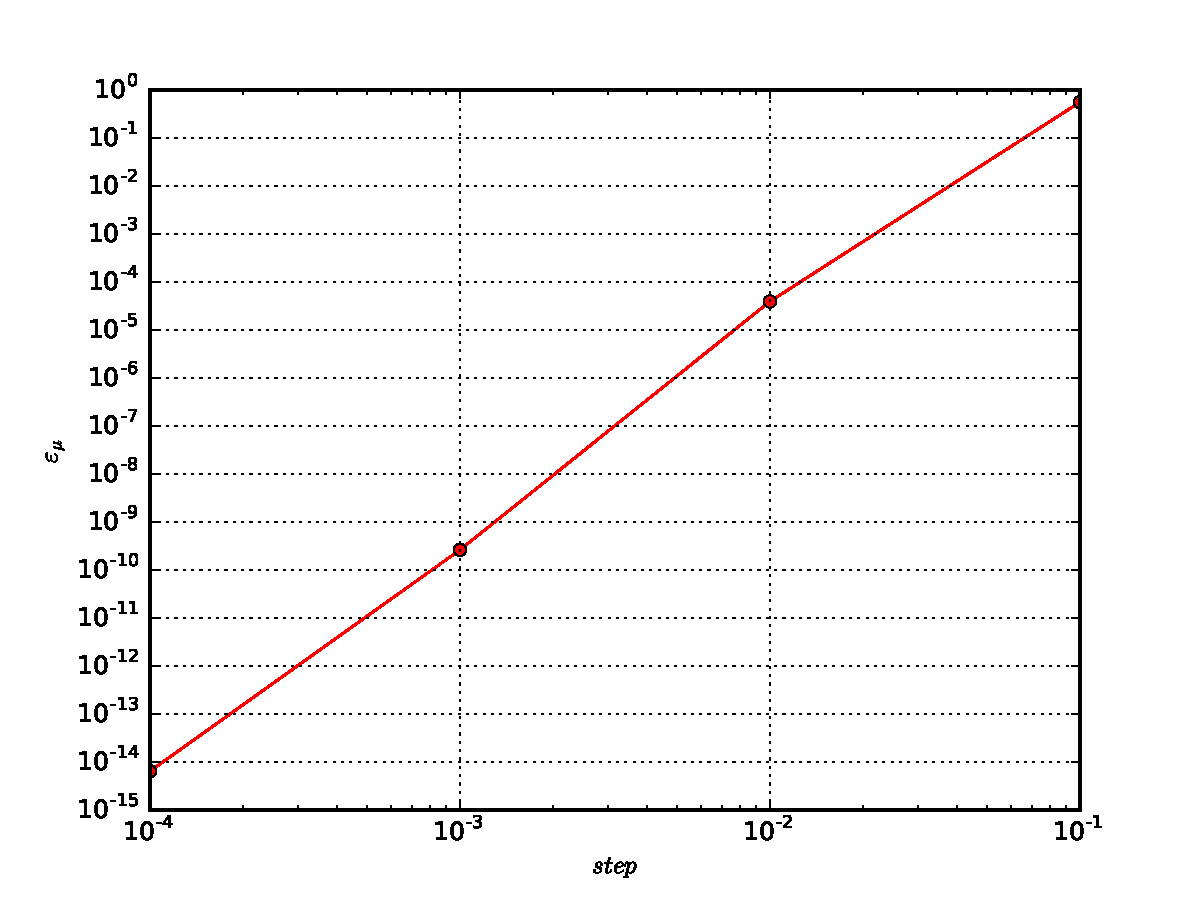
\includegraphics[width=0.75\textwidth]{../pictures/lab5_eigvals_error.pdf}
	\caption{Отклонение модуля собственных чисел матрицы-пропагатора от 1}
	\label{fig:eigvals_error}
\end{figure}

\begin{figure}[H]
	\center
	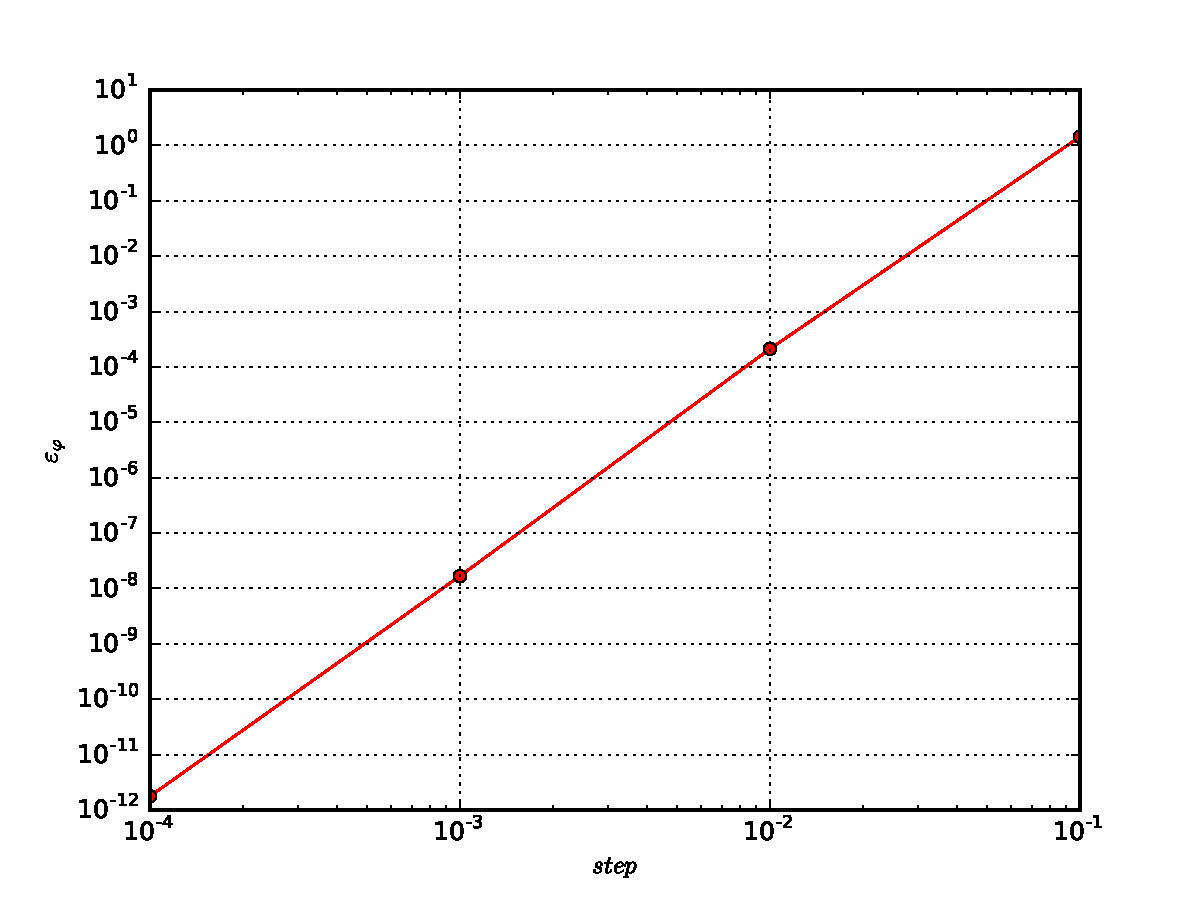
\includegraphics[width=0.75\textwidth]{../pictures/lab5_eigvecs_error.pdf}
	\caption{Оценка ошибки нахождения собственныx векторов матрицы-пропагатора}
	\label{fig:eigvecs_error}
\end{figure}

\section{Количественные характеристики решений уравнения Шрёдингера c
периодическим по времени гамильтонианом}

Для периодического по времени гамильтониана из (\ref{eq:schrodinger_eq}) можно ввести
аналог энегрии стационарной системы: \(E_\alpha(t)=\bra{\varphi_\alpha(t)}H(t)\ket{\varphi_\alpha(t)}\),
где \(\alpha\) --- индекс Флоке-вектора. Будем рассматривать величниу \(E_\alpha(0)\),
тогда \(\varphi_\alpha(0)\) является собственным вектором пропагатора \(U(T)\).

Для изучения распределения величины \(E_\alpha(0)\) (квазиэнергии нестационарной системы)
при значениях \(F\in\{0.01,0.1,1\}\) были сгенерировынны 120 реализаций пар матриц
\((H_0, H_1)\) из (\ref{eq:schrodinger_eq}) размерности 100.
Перед построением нормированных гистограмм, как и в случае стационарной системы,
квазиэнергии были умножены на коэффициент на \(\frac{1}{\sqrt{N}}\), чтобы их спектр
не зависел от размерности системы.

На рис. \ref{fig:floquet_energies_f_0_01}, \ref{fig:floquet_energies_f_0_1}, \ref{fig:floquet_energies_f_1}
можно увидеть, что с ростом \(F\) спектр начинает сосредотачивается в окрестности \(0\)
(то есть при нарастании отличия гамильтониана от стационарного): при \(F=0.01\) спектр
квазиэнергий почти не отличается от спектра энергий стационарной системы, а при \(F=1\)
имеется явный пик распределения вблизи \(0\).

\begin{figure}[H]
	\center
	\includegraphics[width=0.75\textwidth]{../pictures/{lab5_eigens_histF=0.01}.pdf}
	\caption{Распределение энергий Флоке-векторов гамильтониана при \(F=0.01\)}
	\label{fig:floquet_energies_f_0_01}
\end{figure}

\begin{figure}[H]
	\center
	\includegraphics[width=0.75\textwidth]{../pictures/{lab5_eigens_histF=0.1}.pdf}
	\caption{Распределение энергий Флоке-векторов гамильтониана при \(F=0.1\)}
	\label{fig:floquet_energies_f_0_1}
\end{figure}

\begin{figure}[H]
	\center
	\includegraphics[width=0.75\textwidth]{../pictures/{lab5_eigens_histF=1}.pdf}
	\caption{Распределение энергий Флоке-векторов гамильтониана при \(F=1\)}
	\label{fig:floquet_energies_f_1}
\end{figure}

Как и в стационарном случае, наряду с самими квазиэнергиями
рассматривается и их расщепление, определяемое по формуле:
\(s_\alpha = E(0)_{\alpha+1}-E(0)_\alpha, i=\overline{1,N-1}\). По полученным
ранее реализациям были построены гистограммы нормированных расщеплений:
\(\bar s_\alpha =s_\alpha/\langle s \rangle>\), где \(\langle s\rangle\) --- средняя
величина расщепления. Из рис. \ref{fig:floquet_energies_spacing_f_0_01},
\ref{fig:floquet_energies_spacing_f_0_1}, \ref{fig:floquet_energies_spacing_f_1}
видно, что для гамильтониана, близкого к стационарному, распределения имеет удалённый
от нуля пик, но при увеличении \(F\) этот пик смещается влево, что говорит о
росте плотности спектра квазиэнегий.

\begin{figure}[H]
	\center
	\includegraphics[width=0.75\textwidth]{../pictures/{lab5_eigens_spacings_histF=0.01}.pdf}
	\caption{Распределение расщепления энергий Флоке-векторов гамильтониана при \(F=0.01\)}
	\label{fig:floquet_energies_spacing_f_0_01}
\end{figure}

\begin{figure}[H]
	\center
	\includegraphics[width=0.75\textwidth]{../pictures/{lab5_eigens_spacings_histF=0.1}.pdf}
	\caption{Распределение расщепления энергий Флоке-векторов гамильтониана при \(F=0.1\)}
	\label{fig:floquet_energies_spacing_f_0_1}
\end{figure}

\begin{figure}[H]
	\center
	\includegraphics[width=0.75\textwidth]{../pictures/{lab5_eigens_spacings_histF=1}.pdf}
	\caption{Распределение расщепления энергий Флоке-векторов гамильтониана при \(F=1\)}
	\label{fig:floquet_energies_spacing_f_1}
\end{figure}

\section{Исходный код}
\lstinputlisting[language=Python, numbers=left]{../scripts/lab5.py}

\end{document}
